\documentclass{beamer}
\usepackage{graphicx}
\usepackage{fontspec}
\usepackage{polyglossia}
\setdefaultlanguage{russian}

% Определение шрифтов для кириллицы
\newfontfamily\cyrillicfont{Arial} % Замените Arial на доступный шрифт, поддерживающий кириллицу
\setmainfont{Times New Roman} % Основной шрифт для латиницы
\setsansfont{Arial} % Шрифт для без засечек
\setmonofont{Courier New} % Моноширинный шрифт

\title{Техническая и издательская документация}
\author{Зубов Михаил}
\date{\today}

\begin{document}

\frame{\titlepage}

\begin{frame}
\frametitle{Введение}
Техническая и издательская документация — это важные компоненты любой организации, обеспечивающие четкое и понятное представление информации.
\end{frame}

\begin{frame}
\frametitle{Типы документации}
\begin{itemize}
    \item Техническая документация
    \item Пользовательская документация
    \item Научные публикации
    \item Учебные материалы
\end{itemize}
\end{frame}

\begin{frame}
\frametitle{тут картинка}
\begin{figure}
\centering
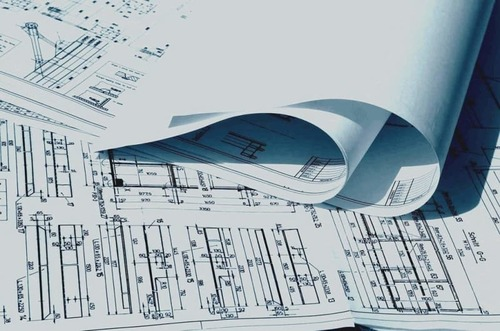
\includegraphics[width=0.8\textwidth]{3.jpg}
\caption{это какая-то документация}
\end{figure}
\end{frame}

\begin{frame}
\frametitle{Техническая документация}
\begin{itemize}
    \item Описание систем и процессов.
    \item Спецификации и требования.
    \item Инструкции по эксплуатации и обслуживанию.
\end{itemize}
\end{frame}

\begin{frame}
\frametitle{Издательская документация}
\begin{itemize}
    \item Книги и журналы.
    \item Научные статьи и исследования.
    \item Редакционные и издательские процессы.
\end{itemize}
\end{frame}

\begin{frame}
\frametitle{Качество документации}
\begin{columns}
\column{0.5\textwidth}
\begin{block}{Показатели качества}
\begin{itemize}
    \item Ясность и доступность.
    \item Полнота и точность.
    \item Актуальность информации.
\end{itemize}
\end{block}
\column{0.5\textwidth}
\begin{block}{Процесс редактирования}
\begin{itemize}
    \item Проверка фактов.
    \item Корректура и стилистическая правка.
    \item Обратная связь от пользователей.
\end{itemize}
\end{block}
\end{columns}
\end{frame}

\begin{frame}
\frametitle{Современные инструменты}
\begin{itemize}
    \item Системы управления документами (DMS).
    \item Программное обеспечение для редактирования и форматирования.
    \item Онлайн-платформы для публикации и распространения.
\end{itemize}
\end{frame}

\begin{frame}
\frametitle{Заключение}
Техническая и издательская документация играют ключевую роль в обеспечении эффективного обмена информацией и поддержании качества продуктов и услуг.
\end{frame}

\begin{frame}
\frametitle{Вопросы?}
Спасибо за внимание! Есть ли у вас вопросы?
\end{frame}

\end{document}


